\documentclass[11pt]{article}

\usepackage[a4paper,margin=1in]{geometry}
\usepackage{amsmath,amssymb,amsthm,mathtools}
\usepackage{xcolor}
\usepackage{listings}
\usepackage{hyperref}
\usepackage{enumitem}
\usepackage{mdframed}
\usepackage{booktabs}
\usepackage{tabularx}
\usepackage{titlesec}
\usepackage{parskip}
\usepackage{graphicx}

\hypersetup{colorlinks=true, linkcolor=blue!50!black, urlcolor=blue!50!black}

\titlespacing*{\section}{0pt}{14pt}{5pt}
\titlespacing*{\subsection}{0pt}{10pt}{4pt}
\setlist{nosep, topsep=3pt, itemsep=3pt}
\setlength{\parskip}{6pt}

\definecolor{codebg}{RGB}{243,242,239}
\definecolor{codekeyword}{RGB}{42,120,214}
\definecolor{codecomment}{RGB}{110,110,110}
\lstset{
  basicstyle=\ttfamily\small, backgroundcolor=\color{codebg},
  keywordstyle=\color{codekeyword}\bfseries, commentstyle=\color{codecomment}\itshape,
  frame=single, breaklines=true, showstringspaces=false, tabsize=4,
  columns=flexible, aboveskip=6pt, belowskip=6pt
}

\newmdenv[backgroundcolor=blue!5, linecolor=blue!40!black, linewidth=0.7pt, roundcorner=3pt,
  innermargin=8pt, outermargin=8pt, innertopmargin=6pt, innerbottommargin=6pt, skipabove=8pt, skipbelow=8pt]{cbox}
\newmdenv[backgroundcolor=green!6, linecolor=green!35!black, linewidth=0.7pt, roundcorner=3pt,
  innermargin=8pt, outermargin=8pt, innertopmargin=6pt, innerbottommargin=6pt, skipabove=8pt, skipbelow=8pt]{keyidea}
\newmdenv[backgroundcolor=gray!7, linecolor=gray!50!black, linewidth=0.6pt, roundcorner=2pt,
  innermargin=8pt, outermargin=8pt, innertopmargin=6pt, innerbottommargin=6pt, skipabove=8pt, skipbelow=8pt]{recap}

\title{\textbf{The fracmem Guide}\\[0.3em]
\large What it is, why it works, and how to use it --- in plain language}
\author{}
\date{\today}

\begin{document}
\maketitle

\begin{cbox}
\textbf{What this document is.} Everything about \texttt{fracmem} in one place, written as simply as possible: the problem it solves, why the solution actually works (with a real proof, kept short), a tiny example you can check by hand, how to use the library, and real measured results. No prior background is assumed.
\end{cbox}

\tableofcontents

%=================================================================
\section{The problem}

A normal derivative only looks at the last one or two readings: ``how fast is this changing \emph{right now}?'' A \textbf{fractional-order derivative} (order $\alpha$, e.g.\ $\alpha=0.5$, a ``half derivative'') is different: computing it exactly needs \textbf{every reading you've ever taken}, not just recent ones. This shows up in fractional-order control, battery models, and materials that ``remember'' how they were stressed years ago.

That's a real problem for any device that runs for a long time: the amount of memory and work needed keeps growing, forever. \texttt{fracmem} exists to fix this: give (almost) the same answer, but using a \emph{fixed} amount of memory and work, no matter how long the device has been running.

%=================================================================
\section{The idea, in one picture}

Picture a row of leaky buckets. Every new reading gets poured into all of them at once. Each bucket leaks at its own fixed rate --- some leak fast (they only ``remember'' the last few readings), some leak very slowly (they still hold a little of what was poured in long ago). Add up what's currently in all the buckets, with the right weight for each bucket, and you get a good stand-in for ``the weighted sum of the entire past'' --- without ever storing the past itself. Just one number per bucket, updated every step.

\begin{keyidea}
That's the whole idea. A fractional derivative needs to remember its whole history because its memory fades as a \textbf{power law} (slowly, e.g.\ $\sim 1/j^{1.5}$). A leaky bucket forgets \emph{geometrically} (fast, e.g.\ $0.9^j$) and can be tracked with one running number. \texttt{fracmem} replaces the slow-fading, expensive-to-track power law with a handful of fast-fading, cheap-to-track leaky buckets, chosen so that together they still add up to (almost) the same answer.
\end{keyidea}

%=================================================================
\section{Why it works --- the proof, kept short}

\subsection{The one fact everything rests on}
A single leaky bucket with leak rate $\lambda$ (a number between 0 and 1) can be updated with one multiply: $\lambda^{j+1} = \lambda \cdot \lambda^j$. Check it: $\lambda=0.9$, $\lambda^3=0.729$, $\lambda^4 = 0.9\times0.729=0.6561$ --- exactly $0.9^4$. You never need to remember $j$ or recompute anything; just keep one number and multiply. A power law $j^{-\beta}$ has \emph{no} such shortcut --- there's no fixed number that turns $j^{-\beta}$ into $(j{-}1)^{-\beta}$, because the ratio keeps changing as $j$ grows. That's the entire reason this approach is worth building: exponentials are cheap to track; power laws are not.

\subsection{The identity that makes the swap possible}
The Gamma function is just the factorial, extended to non-whole numbers: $\Gamma(n)=(n{-}1)!$ for whole $n$ (e.g.\ $\Gamma(4)=3!=6$), and $\Gamma(\beta)=\int_0^\infty x^{\beta-1}e^{-x}dx$ in general. Substituting $x=sj$ into that definition and simplifying gives, exactly:
\[
j^{-\beta} \;=\; \frac{1}{\Gamma(\beta)}\int_0^\infty s^{\beta-1}e^{-sj}\,ds.
\]
In words: the power law on the left is \emph{exactly equal} to a blend of every possible leaky bucket (every decay rate $s$ from 0 to $\infty$) on the right, weighted by $s^{\beta-1}/\Gamma(\beta)$. Nothing is approximated yet.

\subsection{Turning that into a short, real sum}
Two practical steps make this computable:
\begin{itemize}
\item \textbf{Only keep the range of $s$ that matters.} Very small $s$ barely decays at all; very large $s$ decays away almost instantly. Both extremes contribute nothing useful, so they're cut off.
\item \textbf{Pick a handful of representative $s$ values, spaced out on a log scale (not evenly).} The useful range of $s$ spans several orders of magnitude, so evenly-spaced points would waste almost all of them on one end. Log-spacing puts one near every scale that matters.
\end{itemize}
That turns the integral into a short, finite sum: $j^{-\beta} \approx \sum_{i=1}^p c_i\, e^{-s_i j}$, for $p$ chosen decay rates $s_i$ (\texttt{fracmem}'s default is $p=16$ buckets).

\subsection{The guarantee}
Because every $s_i$ (and therefore every bucket's leak rate $\lambda_i = e^{-s_i}$) comes from this exact formula --- never guessed, never fit to any signal --- you can measure \emph{on paper, before ever running the filter on real data} exactly how far the $p$-bucket approximation is from the true power law. \texttt{fracmem} does this with \texttt{soe\_tail\_error(...)}, and Section 5 shows the real number this gives.

\subsection{Why only one half gets touched by data}
The final piece uses a small amount of real training data --- but only to adjust \emph{how much weight} each bucket gets ($c_i$), never the leak rates ($\lambda_i$) themselves. Why the split: $\lambda_i$ already has an exact, known-correct answer (the formula above) --- there is nothing for real data to improve, and trying to re-derive it from noisy examples can only make it worse. $c_i$ has no such closed form (it depends on exactly how the local window and the buckets interact for real signals), so a small, well-behaved linear fit against real examples genuinely helps there. This is a deliberate design choice with its own justification, not an oversight, and it also keeps the fitting problem simple: adjusting only $c_i$ (with $\lambda_i$ fixed) is an ordinary, always-solvable linear regression, not a fragile, many-local-optima search.

\begin{recap}
\textbf{In one paragraph:} a power law can be written, exactly, as a blend of every possible exponential decay rate (the Gamma-function identity). Picking a handful of representative rates, log-spaced, turns that into a short, real sum --- a few leaky buckets that together approximate the whole slow-fading memory. Because the rates come from an exact formula, the worst-case error is knowable in advance. Only the buckets' combination weights get refined with a little real data, because that's the only part with no closed-form answer.
\end{recap}

%=================================================================
\section{A tiny example you can check by hand}
Take $\alpha=0.5$ and just 3 buckets (the real library uses 16; three is enough to see the mechanism). Every number below comes straight from the formulas above:

\begin{table}[h]
\centering
\small
\begin{tabular}{cccc}
\toprule
bucket $i$ & decay rate $s_i$ & leak rate $\lambda_i = e^{-s_i}$ & weight $c_i$ \\
\midrule
0 & 0.004472 & 0.995538 & $2.47\times10^{-4}$ \\
1 & 0.089443 & 0.914441 & $1.46\times10^{-3}$ \\
2 & 1.788854 & 0.167152 & $3.15\times10^{-25}$ \\
\bottomrule
\end{tabular}
\end{table}

Bucket 0 leaks almost nothing per step (long memory); bucket 2 leaks almost everything per step (short memory, and its weight underflows to near-zero here simply because it's so far from where the local window ends). Together, even just these three already stand in for a power law that nominally needs the entire past.

%=================================================================
\section{What the real code actually achieves}
Three buckets is for intuition. Running the real code with \texttt{fracmem}'s actual default ($p=16$, $\alpha=0.5$) and comparing the 16-bucket approximation against the true, exact kernel weights gives:

\begin{table}[h]
\centering
\small
\begin{tabular}{rrr}
\toprule
how far back & true weight & how far off the approximation is \\
\midrule
64 samples   & $-5.542\times10^{-4}$ & 0.013\% \\
256 samples  & $-6.897\times10^{-5}$ & 0.028\% \\
1000 samples & $-8.924\times10^{-6}$ & 0.011\% \\
4000 samples & $-1.115\times10^{-6}$ & 0.340\% \\
\bottomrule
\end{tabular}
\end{table}

Worst case across the whole range: \textbf{0.34\% error} --- 16 numbers standing in for a sum that would otherwise need every one of thousands of past samples. This is a real, measured number from actually running \texttt{soe\_tail\_kernel} in \texttt{soe.py}, not an estimate.

%=================================================================
\section{How to use it}

\begin{lstlisting}[language=bash]
pip install git+https://github.com/edith-lang/fracmem.git
\end{lstlisting}

\begin{lstlisting}[language=Python]
import numpy as np
from fracmem import CompressedFractionalFilter

f = CompressedFractionalFilter(alpha=0.5, h=0.01, L=32, p=16)

train_signals = [np.random.randn(3000).cumsum() * 0.01 for _ in range(8)]
f.fit(train_signals)            # done once, offline

new_signal = np.random.randn(50_000).cumsum() * 0.01
y_hat = f.predict(new_signal)   # fixed cost per sample, however long the signal is
\end{lstlisting}

\begin{table}[h]
\centering
\small
\begin{tabularx}{\textwidth}{lX}
\toprule
Call & What it does \\
\midrule
\texttt{.fit(signals)} & Learn the bucket weights $c_i$ from example signals (the leak rates $\lambda_i$ come from pure math, always). \\
\texttt{.predict(x)} & Run the fitted filter over a whole array at once. \\
\texttt{.step(x\_k)} & Feed one new sample at a time --- for a live, streaming use case. \\
\texttt{.from\_analytic(...)} & Build a working filter with \emph{zero} training data, pure math only. \\
\texttt{fracmem.embedded.export\_micropython(...)} & Bake a fitted filter into a standalone file for an ESP32/MicroPython board. \\
\texttt{fracmem.embedded.export\_c(...)} & Bake a fitted filter into plain C, for any real C/C++ embedded toolchain. \\
\bottomrule
\end{tabularx}
\end{table}

%=================================================================
\section{Real-world results}
A separate, real GPU benchmark (see \texttt{benchmarks/BENCHMARKS.md} in the repository for full detail and how to reproduce it) tested \texttt{fracmem} against a hand-verified, honest exact reference --- five times, at five different amounts of training data, all on the same 5,000,000-sample test signal:

\begin{center}
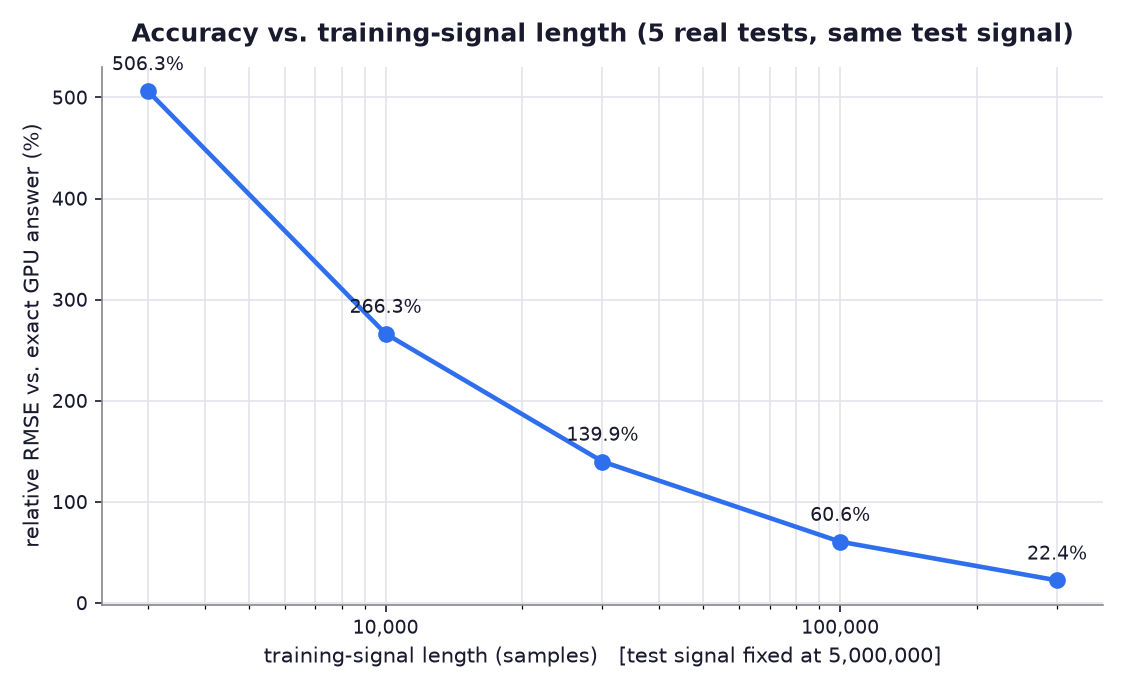
\includegraphics[width=0.85\textwidth]{accuracy_vs_train_length.png}
\end{center}

\begin{itemize}
\item Accuracy improves steadily and predictably as training data grows --- 506\% error with almost no training data, down to 22\% with a healthy amount.
\item The compiled-C version ran \textbf{159--171$\times$ faster} than the exact reference, consistently, across every test.
\item An unexpected but real finding: at very long deployments, the compiled C version's lower numeric precision (needed to keep it cheap on a small device) can itself become the accuracy limit, once training is already good. Details and the fix are in \texttt{benchmarks/}\-\texttt{BENCHMARKS.md}.
\end{itemize}

%=================================================================
\section{Where to look in the code}
\begin{table}[h]
\centering
\small
\begin{tabularx}{\textwidth}{lX}
\toprule
File & What's in it \\
\midrule
\texttt{kernel.py} & The exact, expensive definition (Section 1) --- the target everything else approximates. \\
\texttt{soe.py} & The leaky-bucket construction (Sections 3--4): pure math, no data. \\
\texttt{filter.py} & \texttt{CompressedFractionalFilter}: fitting, predicting, streaming. \\
\texttt{embedded/} & MicroPython and plain-C export for real devices. \\
\bottomrule
\end{tabularx}
\end{table}

\end{document}
